% Options for packages loaded elsewhere
% Options for packages loaded elsewhere
\PassOptionsToPackage{unicode}{hyperref}
\PassOptionsToPackage{hyphens}{url}
\PassOptionsToPackage{dvipsnames,svgnames,x11names}{xcolor}
%
\documentclass[
  article]{jss}
\usepackage{xcolor}
\usepackage{amsmath,amssymb}
\setcounter{secnumdepth}{5}
\usepackage{iftex}
\ifPDFTeX
  \usepackage[T1]{fontenc}
  \usepackage[utf8]{inputenc}
  \usepackage{textcomp} % provide euro and other symbols
\else % if luatex or xetex
  \usepackage{unicode-math} % this also loads fontspec
  \defaultfontfeatures{Scale=MatchLowercase}
  \defaultfontfeatures[\rmfamily]{Ligatures=TeX,Scale=1}
\fi
\usepackage{lmodern}
\ifPDFTeX\else
  % xetex/luatex font selection
\fi
% Use upquote if available, for straight quotes in verbatim environments
\IfFileExists{upquote.sty}{\usepackage{upquote}}{}
\IfFileExists{microtype.sty}{% use microtype if available
  \usepackage[]{microtype}
  \UseMicrotypeSet[protrusion]{basicmath} % disable protrusion for tt fonts
}{}
\makeatletter
\@ifundefined{KOMAClassName}{% if non-KOMA class
  \IfFileExists{parskip.sty}{%
    \usepackage{parskip}
  }{% else
    \setlength{\parindent}{0pt}
    \setlength{\parskip}{6pt plus 2pt minus 1pt}}
}{% if KOMA class
  \KOMAoptions{parskip=half}}
\makeatother
% Make \paragraph and \subparagraph free-standing
\makeatletter
\ifx\paragraph\undefined\else
  \let\oldparagraph\paragraph
  \renewcommand{\paragraph}{
    \@ifstar
      \xxxParagraphStar
      \xxxParagraphNoStar
  }
  \newcommand{\xxxParagraphStar}[1]{\oldparagraph*{#1}\mbox{}}
  \newcommand{\xxxParagraphNoStar}[1]{\oldparagraph{#1}\mbox{}}
\fi
\ifx\subparagraph\undefined\else
  \let\oldsubparagraph\subparagraph
  \renewcommand{\subparagraph}{
    \@ifstar
      \xxxSubParagraphStar
      \xxxSubParagraphNoStar
  }
  \newcommand{\xxxSubParagraphStar}[1]{\oldsubparagraph*{#1}\mbox{}}
  \newcommand{\xxxSubParagraphNoStar}[1]{\oldsubparagraph{#1}\mbox{}}
\fi
\makeatother


\usepackage{longtable,booktabs,array}
\usepackage{calc} % for calculating minipage widths
% Correct order of tables after \paragraph or \subparagraph
\usepackage{etoolbox}
\makeatletter
\patchcmd\longtable{\par}{\if@noskipsec\mbox{}\fi\par}{}{}
\makeatother
% Allow footnotes in longtable head/foot
\IfFileExists{footnotehyper.sty}{\usepackage{footnotehyper}}{\usepackage{footnote}}
\makesavenoteenv{longtable}
\usepackage{graphicx}
\makeatletter
\newsavebox\pandoc@box
\newcommand*\pandocbounded[1]{% scales image to fit in text height/width
  \sbox\pandoc@box{#1}%
  \Gscale@div\@tempa{\textheight}{\dimexpr\ht\pandoc@box+\dp\pandoc@box\relax}%
  \Gscale@div\@tempb{\linewidth}{\wd\pandoc@box}%
  \ifdim\@tempb\p@<\@tempa\p@\let\@tempa\@tempb\fi% select the smaller of both
  \ifdim\@tempa\p@<\p@\scalebox{\@tempa}{\usebox\pandoc@box}%
  \else\usebox{\pandoc@box}%
  \fi%
}
% Set default figure placement to htbp
\def\fps@figure{htbp}
\makeatother





\setlength{\emergencystretch}{3em} % prevent overfull lines

\providecommand{\tightlist}{%
  \setlength{\itemsep}{0pt}\setlength{\parskip}{0pt}}





\usepackage{orcidlink,thumbpdf,lmodern}

\newcommand{\class}[1]{`\code{#1}'}
\newcommand{\fct}[1]{\code{#1()}}
\makeatletter
\@ifpackageloaded{caption}{}{\usepackage{caption}}
\AtBeginDocument{%
\ifdefined\contentsname
  \renewcommand*\contentsname{Table of contents}
\else
  \newcommand\contentsname{Table of contents}
\fi
\ifdefined\listfigurename
  \renewcommand*\listfigurename{List of Figures}
\else
  \newcommand\listfigurename{List of Figures}
\fi
\ifdefined\listtablename
  \renewcommand*\listtablename{List of Tables}
\else
  \newcommand\listtablename{List of Tables}
\fi
\ifdefined\figurename
  \renewcommand*\figurename{Figure}
\else
  \newcommand\figurename{Figure}
\fi
\ifdefined\tablename
  \renewcommand*\tablename{Table}
\else
  \newcommand\tablename{Table}
\fi
}
\@ifpackageloaded{float}{}{\usepackage{float}}
\floatstyle{ruled}
\@ifundefined{c@chapter}{\newfloat{codelisting}{h}{lop}}{\newfloat{codelisting}{h}{lop}[chapter]}
\floatname{codelisting}{Listing}
\newcommand*\listoflistings{\listof{codelisting}{List of Listings}}
\makeatother
\makeatletter
\makeatother
\makeatletter
\@ifpackageloaded{caption}{}{\usepackage{caption}}
\@ifpackageloaded{subcaption}{}{\usepackage{subcaption}}
\makeatother
\makeatletter
\@ifpackageloaded{tcolorbox}{}{\usepackage[skins,breakable]{tcolorbox}}
\makeatother
\makeatletter
\@ifundefined{shadecolor}{\definecolor{shadecolor}{rgb}{.97, .97, .97}}{}
\makeatother
\makeatletter
\makeatother
\makeatletter
\ifdefined\Shaded\renewenvironment{Shaded}{\begin{tcolorbox}[borderline west={3pt}{0pt}{shadecolor}, sharp corners, interior hidden, frame hidden, enhanced, breakable, boxrule=0pt]}{\end{tcolorbox}}\fi
\makeatother
\usepackage{bookmark}
\IfFileExists{xurl.sty}{\usepackage{xurl}}{} % add URL line breaks if available
\urlstyle{same}
\hypersetup{
  pdftitle={A Framework for Reproducible Data Science using Nix},
  pdfauthor={Bruno Rodrigues},
  pdfkeywords={reproducibility, R, Nix},
  colorlinks=true,
  linkcolor={blue},
  filecolor={Maroon},
  citecolor={Blue},
  urlcolor={Blue},
  pdfcreator={LaTeX via pandoc}}


%% -- Article metainformation (author, title, ...) -----------------------------

%% Author information
\author{Bruno Rodrigues~\orcidlink{0000-0002-3211-3689}\\Ministry of
Research and Higher education, Luxembourg}
\Plainauthor{Bruno Rodrigues} %% comma-separated

\title{A Framework for Reproducible Data Science using Nix}
\Plaintitle{A Framework for Reproducible Data Science using
Nix} %% without formatting

%% an abstract and keywords
\Abstract{To create a reproducible analysis, it is not enough to write
clean, well-documented and tested code. One must also ensure that all
software dependencies are clearly declared and, ideally, provide a
simple way to install them. Several tools exist for this purpose, such
as the containerization solution \pkg{Docker}. A complete solution,
however, requires not only managing the computational environment but
also orchestrating the execution of the analysis itself in a robust and
automated way. This paper presents a comprehensive framework based on
the \pkg{Nix} package manager to solve both problems. We first introduce
the \proglang{R} package \pkg{rix}, which simplifies the creation of
reproducible environments with \pkg{Nix}. We then introduce
\pkg{rixpress}, a second \proglang{R} package that leverages these
environments to define and execute complex, multi-language analytical
pipelines. Together, these tools provide a powerful, unified approach to
achieving high standards of computational reproducibility.}

%% at least one keyword must be supplied
\Keywords{reproducibility, \proglang{R}, \pkg{Nix}}
\Plainkeywords{reproducibility, R, Nix}

%% publication information
%% NOTE: Typically, this can be left commented and will be filled out by the technical editor
%% \Volume{50}
%% \Issue{9}
%% \Month{June}
%% \Year{2012}
%% \Submitdate{2012-06-04}
%% \Acceptdate{2012-06-04}
%% \setcounter{page}{1}
%% \Pages{1--xx}

%% The address of (at least) one author should be given
%% in the following format:
\Address{
Bruno Rodrigues\\
Department of Statistics\\
18, Montée de la Pétrusse\\
Luxembourg Luxembourg\\
E-mail: \email{bruno@brodrigues.co}\\
URL: \url{https://www.brodrigues.co}\\
\\~

}

\begin{document}
\maketitle


\section{Introduction: Reproducibility is also about
software}\label{sec-intro}

\citet{peng2011} introduced the concept of reproducibility as a
\emph{continuum}. At one end lies the least reproducible state, where
only a paper describing the study is available. Reproducibility improves
when authors share the original source code, improves further when they
include the underlying data, and reaches its highest level when what
Roger Peng called \emph{linked and executable code and data} are
provided.

By \emph{linked and executable code and data}, Peng referred to compiled
source code and runnable scripts. In this paper, we interpret this
notion more broadly as the \emph{computational environment}: the
complete set of software required to execute an analysis. Here too, a
continuum exists. At the minimal end, authors might only name the main
software used---say, the \proglang{R} programming language. More careful
authors might also specify the version of \proglang{R}, or list the
additional packages and their versions. Rarely, however, do authors
specify the operating system on which the analysis was performed, even
though differences in operating systems can lead to divergent results
when using the same code and software versions, as shown by
\citet{neupane2019}. It is even less common for authors to provide
step-by-step installation instructions for the required software stack.

Even when such instructions are given, they often fail across different
platforms or versions of the same platform. This lack of portability not
only hinders reproducibility but also complicates everyday research
workflows. Researchers working across multiple machines must be able to
recreate the same environment consistently, and collaborators must share
identical computational setups to avoid inconsistencies.

Finally, once the execution environment is correctly configured,
additional clarity is needed on how to \emph{run} the project itself.
Which packages should be loaded first? Which scripts should be executed,
and in what order? Without clear documentation or a logically organized
project structure, these operational details become yet another barrier
to reproducibility.

A range of tools now exist to help researchers approach the gold
standard of full reproducibility, or to consistently deploy the same
development environment across multiple machines. Let us first consider
the most basic step in this process: listing the software used. In
\proglang{R}, the \texttt{sessionInfo()} function provides a concise
summary of the software environment, including the R version, platform
details, and all loaded packages. Its output can be saved to a file and
included as part of a study's reproducibility record. Below is an
example output from \texttt{sessionInfo()}:

\begin{CodeInput}
R> sessionInfo()
\end{CodeInput}
\begin{CodeOutput}
R version 4.3.2 (2023-10-31)
Platform: aarch64-unknown-linux-gnu (64-bit)
Running under: Ubuntu 22.04.3 LTS

Matrix products: default
BLAS:   /usr/lib/aarch64-linux-gnu/openblas-pthread/libblas.so.3
LAPACK: /usr/lib/aarch64-linux-gnu/openblas-pthread/libopenblasp[...]

locale:
 LC_CTYPE=en_US.UTF-8       LC_NUMERIC=C              
 LC_TIME=en_US.UTF-8        LC_COLLATE=en_US.UTF-8    
 LC_MONETARY=en_US.UTF-8    LC_MESSAGES=en_US.UTF-8   
 LC_PAPER=en_US.UTF-8       LC_NAME=C                 
 LC_ADDRESS=C               LC_TELEPHONE=C            
 LC_MEASUREMENT=en_US.UTF-8 LC_IDENTIFICATION=C       

time zone: Etc/UTC
tzcode source: system (glibc)

attached base packages:
 stats     graphics  grDevices utils     datasets  methods   base     

other attached packages:
 nnet_7.3-19  mgcv_1.9-0   nlme_3.1-163

loaded via a namespace (and not attached):
 compiler_4.3.2  Matrix_1.6-1.1  tools_4.3.2     splines_4.3.2
 grid_4.3.2      lattice_0.21-9 
\end{CodeOutput}

When an author includes this information, others attempting to reproduce
the study (future readers, collaborators, or even the author at a later
time) can easily see which version of \proglang{R} and which packages
(with their versions) were used. However, reproducing the environment
still requires manually installing the correct package versions. This
can be difficult, especially when packages depend on system-level
libraries. For example, the \pkg{nloptr} package requires a precompiled
\proglang{nlopt} binary, or alternatively, \proglang{cmake} when
building from source on Linux or macOS.

A more robust approach than simply listing package versions is to use
the \pkg{renv} package. \pkg{renv} captures the project's software state
and writes it to a \texttt{renv.lock} file, which includes the exact
versions of \proglang{R} and all required packages. This lockfile serves
as a blueprint for restoring the environment automatically, ensuring
that others can recreate the same setup with minimal effort. Below is an
example of an \texttt{renv.lock} file:

\begin{Code}
{
  "R": {
    "Version": "4.2.2",
    "Repositories": [
      {
        "Name": "CRAN",
        "URL": "https://packagemanager.rstudio.com/all/latest"
      }
    ]
  },
  "Packages": {
    "MASS": {
      "Package": "MASS",
      "Version": "7.3-58.1",
      "Source": "Repository",
      "Repository": "CRAN",
      "Hash": "762e1804143a332333c054759f89a706",
      "Requirements": []
    },
    "Matrix": {
      "Package": "Matrix",
      "Version": "1.5-1",
      "Source": "Repository",
      "Repository": "CRAN",
      "Hash": "539dc0c0c05636812f1080f473d2c177",
      "Requirements": [
        "lattice"
      ]
    }
    
    ... lines below omitted ...
  }
}
\end{Code}

This lockfile lists each package alongside its version and the
repository from which it was downloaded. Creating it requires only a
single command: \texttt{renv::init()}. Others can then reproduce the
same package library by running \texttt{renv::restore()}, which installs
the exact package versions in an isolated, project-specific library that
does not interfere with the user's global R library.

However, \pkg{renv} does not restore the version of \proglang{R} itself.
Installing the correct R version must therefore be done separately.
Similarly, \texttt{renv} does not handle system-level dependencies such
as \proglang{cmake}, which is required by \pkg{nloptr} on Linux and
macOS. These dependencies must be managed manually or through other
tools. Further details are discussed in the \pkg{renv} documentation:
\url{https://rstudio.github.io/renv/articles/renv.html#caveats}.

Before continuing, it should be noted that other packages exist which
provide similar functionality to \pkg{renv}: there is \pkg{groundhog} by
\citet{simonsohn2023} which makes it rather easy to install packages as
they were on CRAN at a given date. For example, the code snippet below
installs the \pkg{purrr} and \pkg{ggplot2} packages as they were on
April 4th, 2017:

\begin{CodeInput}
R> groundhog.library("
+   library('purrr')
+   library('ggplot2')",
+   "2017-10-04",
+   tolerate.R.version = "4.2.2")
\end{CodeInput}

Packages installed with \pkg{groundhog} are placed in a project-specific
library, ensuring they do not interfere with other versions of the same
packages used in different projects. Since \pkg{groundhog} does not
install \proglang{R} itself, users must either install the required R
version manually or use the \texttt{tolerate.R.version} argument, as
illustrated in the example above. Without this argument, \pkg{groundhog}
will not proceed with package installation if the R version does not
match the expected one.

An alternative to \pkg{renv} is \pkg{rang}, developed by
\citet{chan2023}, which similarly allows users to install packages as
they existed on a specific date. Another approach is to use the Posit
Package Manager, which provides dated snapshots of CRAN. For instance,
to ensure that packages are installed as they were on June 30, 2023, one
could include the following line in the \texttt{.Rprofile} file:

\begin{CodeInput}
R> options(repos =
+    c(REPO_NAME =
+      "https://packagemanager.posit.co/cran/__linux__/jammy/2023-06-30"
+    )
+  )
\end{CodeInput}

The \texttt{.Rprofile} file is read by \proglang{R} at the start of each
new session, meaning that every call to \texttt{install.packages()} will
install packages from the specified snapshot mirror. However, unless
users explicitly manage separate libraries for different projects, the
Posit Package Manager will install all packages for all projects as they
existed on that snapshot date.

The next step toward the gold standard of reproducibility is ensuring
not only that the correct package versions are installed, but also that
the correct version of \proglang{R} itself is used. While this can be
done manually, dedicated tools make the process more efficient. One such
tool is \pkg{rig}, developed by the \proglang{R} Infrastructure Team
\citeyearpar{rlib2023}. \pkg{rig} simplifies installing and managing
multiple R versions, allowing users to match the exact version needed
for a given analysis. Once the correct R version is installed, one can
then use tools such as \pkg{renv}, \pkg{groundhog}, or \pkg{rang} to
recreate the associated package library.

However, this multi-step process remains manual, error-prone, and
time-consuming, highlighting the need for more comprehensive and
automated solutions to achieve full computational reproducibility.

The final tool for achieving the gold standard of reproducibility is to
bundle the exact version of \proglang{R} and its packages within a
\pkg{Docker} image. \pkg{Docker} is a containerization platform that
allows packaging a \emph{data product} together with all its
dependencies into a self-contained image. A statistical analysis can be
viewed as such a data product, requiring a specific set of software
dependencies to run. \emph{Dockerizing} an analysis involves building an
image that installs these dependencies, often using the tools mentioned
earlier, and includes the analysis scripts and data (but data can also
be dynamically made available at run-time, to avoid having to copy it
inside the image). The steps to create this image are specified in a
simple text file called a \texttt{Dockerfile}, which defines the
structure and content of the \pkg{Docker} image.

Once the image is built, the analysis can be executed inside a
\emph{container}, which is a running instance of the image. Containers
are typically run non-interactively, allowing the complete computational
environment to be instantiated and executed with a single command.

The strength of \pkg{Docker} lies not only in its ability to encapsulate
the correct versions of \proglang{R} and its packages but also in its
inclusion of system-level dependencies. Since \pkg{Docker} images are
nearly complete Linux systems, they naturally bundle libraries and tools
required by certain R packages (for example, \pkg{nloptr}'s dependency
on the \proglang{nlopt} library). This ensures that future replicators
of a study have access to the same software environment, including all
necessary system components. Moreover, these images can be easily
shared, enabling seamless reproducibility across machines and
collaborators.

The Rocker project, introduced by \citet{boettiger2017}, provides a
collection of pre-built \pkg{Docker} images for the \proglang{R}
community. These images come with specific R versions and, in some
cases, preinstalled packages, making them convenient base images for
building reproducible analysis environments without starting from
scratch.

Despite its strengths, \pkg{Docker} can be cumbersome for interactive
use. Although containers can be modified at runtime, any changes are
lost once the container stops unless they are explicitly saved. Running
graphical applications from containers is also possible, but it is
generally difficult to configure and tends to work reliably only on
Linux systems. For this reason, \pkg{Docker} is most often used to run
web-based applications (such as integrated development environments,
IDEs, like the web version of RStudio) inside containers, offering a
reproducible yet flexible environment for interactive work.

Some IDEs provide built-in support for executing code directly within a
running container, allowing a more seamless workflow. However, these
setups typically require additional configuration, and many
general-purpose IDEs are not well optimized for statistical or data
science workflows (though Positron may soon change that).

A common practice is to conduct a study interactively using a standard
installation of \proglang{R} and its packages, and only after completing
the analysis, create a \texttt{Dockerfile} to allow others to reproduce
the results easily. For instance, the \pkg{dockerfiler} package
\citep{dockerfiler} can automatically generate a \texttt{Dockerfile}
from an existing \texttt{renv.lock} file, simplifying this process.
While this approach enables post-hoc reproducibility, it does not solve
the challenge of consistently deploying the same environment across
multiple machines as co-authors are working on the project. Ideally,
analyses would be developed directly within a containerized environment
from the start, ensuring that the computational setup is reproducible
throughout the project lifecycle.

Another challenge of using \pkg{Docker} is that its images are
effectively minimal Linux systems, so familiarity with Linux is highly
recommended for writing reliable and efficient \texttt{Dockerfile}s. To
guarantee that a build consistently produces the same image, the
\texttt{Dockerfile} should reference specific image \emph{digests}
rather than general \emph{tags}. In practice, however, tagged versions
are more commonly used, which can introduce potential reproducibility
issues. \pkg{dockerfiler} is an R package that lowers the barrier to
entry by automating parts of the \texttt{Dockerfile} creation process,
but they cannot fully replace the need for basic Linux knowledge.

A final step toward the gold standard of reproducibility is to automate
the analysis execution using a build system such as \pkg{Make}, rather
than relying on ad hoc script execution. Build automation tools enable
analyses to be defined as a series of reproducible, well-ordered steps
that can be executed consistently. Within \proglang{R}, a modern and
powerful alternative is the \pkg{targets} package by \citet{landau2021},
which provides declarative workflows for reproducible data analysis.

\citet{mcdermott2021} provides a clear example of a scientific study
that achieved the gold standard of reproducibility. The author created
an accompanying GitHub repository\footnote{https://github.com/grantmcdermott/skeptic-priors}
containing detailed instructions to install the required software and
execute the analysis. Examining this repository reveals the use of
multiple tools to capture and share the computational environment:

\begin{itemize}
\tightlist
\item
  Packages and their versions were recorded in an \texttt{renv.lock}
  file;
\item
  A \texttt{Makefile} was used to automate the full analysis and compile
  the paper;
\item
  A \texttt{Dockerfile} provided a complete computational environment,
  including the correct version of \proglang{R}, enabling easy execution
  of the entire workflow.
\end{itemize}

Reaching this gold standard, however, is resource-intensive. It requires
learning a tool for managing package versions, mastering \pkg{Docker}
for the programming language and other software dependencies, and using
a build automation tool. Importantly, these considerations are not
unique to \proglang{R}: similar approaches are needed for
\proglang{Python} or any other programming language, and complexity
further increases if several programming languages are needed for a
single project.

As an alternative, we present the \pkg{Nix} package manager, which
supports all major operating systems and emphasizes reproducible
software installation and building. \pkg{Nix} can replace \pkg{Docker},
\pkg{renv}, and even build automation tools such as \pkg{Make}. To make
\pkg{Nix} more accessible for \proglang{R} users, we developed the
\pkg{rix} and {rixpress} packages, which are introduced and discussed in
this article.

\section{The Nix package manager}\label{sec-nix}

\pkg{Nix} is a package manager designed to install and build software in
a fully reproducible manner. As of this writing, it provides access to
over 120000 packages, including nearly all of CRAN and Bioconductor.
This allows users to install not only \proglang{R} itself but also all
packages required for a given project. Although \pkg{Nix} is the package
manager of the NixOS Linux distribution, it can also be installed as a
standalone tool on other Linux distributions, macOS, and the Windows
Subsystem for Linux\footnote{Effectively treating non-NixOS Linux
  distributions and Windows as equivalent platforms in practice.}.

The advantage of using \pkg{Nix} to install \proglang{R} packages,
instead of the standard \texttt{install.packages()} function, is that
\pkg{Nix} ensures all dependencies of each package are installed,
whether they are other \proglang{R} packages or system-level libraries.

For example, the \pkg{xlsx} package requires \proglang{Java} to be
installed. On some systems, installing \proglang{Java} may be difficult
or even impossible manually. With \pkg{Nix}, however, the user only
needs to declare that \pkg{xlsx} is required for the project; \pkg{Nix}
automatically installs and configures \proglang{Java} as a dependency.
This works because the maintainers of the \proglang{R} language packages
for \pkg{Nix} have declared \proglang{Java} as a dependency of
\pkg{xlsx}, allowing the process to happen seamlessly from the end-user
perspective.

\pkg{xlsx} can thus be referred to as a component closure, and quoting
\citet{dolstra2004nix}:

\begin{quote}
The idea is to always deploy component closures: if we deploy a
component, then we must also deploy its dependencies, their
dependencies, and so on. That is, we must always deploy a set of
components that is closed under the `'depends on'\,' relation. Since
closures are selfcontained, they are the units of complete software
deployment. After all, if a set of components is not closed, it is not
safe to deploy, since using them might cause other components to be
referenced that are missing on the target system.
\end{quote}

But how does \pkg{Nix} achieve this reproducibility? Where do these
packages, or \emph{closures}, come from? When installing a package with
\pkg{Nix}, an expression written in the \pkg{Nix} language is downloaded
from the \texttt{nixpkgs} GitHub repository and evaluated. These
expressions define \emph{derivations}, which describe how to build a
package: specifying its dependencies, the commands to build and install
it, and the resulting output. Typically, a derivation downloads the
source code, compiles it, and outputs a binary. Derivations are highly
flexible; by writing custom derivations, users can define and build
reproducible environments instead of a single program. The dependencies
of each derivation are themselves defined in other expressions and are
automatically installed if needed. In the case of \proglang{R},
maintainers declare the appropriate dependencies to create fully
self-contained component closures.

Why is installing software with \pkg{Nix} reproducible? Because the
entire set of \pkg{Nix} expressions is hosted on GitHub, it is possible
to reference a specific commit of \texttt{nixpkgs}, a process called
\emph{pinning a revision}. Pinning a revision ensures that all packages
installed by \pkg{Nix} are always the exact same versions, regardless of
when in the future they are built, since the expressions downloaded
correspond to that specific commit of \texttt{nixpkgs}.

Pinning is crucial, but it is not the only reason \pkg{Nix} supports
reproducibility. \pkg{Nix} is a functional package manager: it applies
principles from functional programming, disallowing side effects and
global variables, and ensuring that the output of a build is always the
same given the same inputs, regardless of time or location. A side note:
while this functional approach greatly enhances reproducibility, it can
make writing derivations more complex, particularly for packages that
need to download assets during installation (e.g., some Bioconductor
packages like \pkg{musData}). However, this concern is primarily for
package maintainers, not end-users.

Additionally, \pkg{Nix} supports multiple versions, or \emph{variants},
of a package on the same system. Each variant has a unique identifier,
allowing multiple versions of \proglang{R} to coexist and ensuring the
correct version is used for each project. For a more technical
discussion of \pkg{Nix}, we refer to \citet{dolstra2004nix}.

With \pkg{Nix}, it is possible to effectively replace both \pkg{renv}
and \pkg{Docker} for \proglang{R} projects---or, in the case of
\proglang{Python}, to replace \texttt{requirements.txt} files and
virtual environments. \pkg{Nix} also supports building multi-language
environments, which can include \proglang{R} and \proglang{Python}, a
\LaTeX distribution or any other of the 120,000 available tools. This
enables the creation of a complete, project-specific, and reproducible
environment that can be used interactively or non-interactively. As long
as the \texttt{nixpkgs} GitHub repository remains online, the
environment can be rebuilt in the future to rerun analyses reliably.

However, \pkg{Nix} has a steep learning curve. It is a complex system
that comes with its own programming language, also called
\proglang{Nix}, designed to solve the challenging problem of
declaratively defining how software is built and configured. This
ensures that installations are fully reproducible across operating
systems and hardware platforms. To make \pkg{Nix} more accessible to
\proglang{R} users that wish to use project-specific and reproducible
development environments, we developed the \pkg{rix} package.

\section{Reproducible development environments with
Nix}\label{sec-repro-nix}

As mentioned, \pkg{Nix} expressions are written in the \proglang{Nix}
programming language, which is purely functional. Here is a simple
example that creates a shell environment containing version 4.3.1 of
\proglang{R}:

\begin{CodeInput}
let
  pkgs = import (fetchTarball
    "https://github.com/NixOS/nixpkgs/archive/976fa336.tar.gz"
  ) {};
  system_packages = builtins.attrValues {
    inherit (pkgs) R;
  };
in
  pkgs.mkShell {
    buildInputs = [ system_packages ];
    shellHook = "R --vanilla";
  }
\end{CodeInput}

In this expression, the \texttt{let} keyword is used to define
variables. The variable \texttt{pkgs} imports the set of packages from
the \texttt{nixpkgs} repository at the specified commit
\texttt{976fa336}. The variable \texttt{system\_packages} lists the
packages to include in the environment; in this case, it is just the
\proglang{R} programming language, along with all its dependencies and
their transitive dependencies. The \texttt{mkShell} function then
creates a development shell with the specified packages. The
\texttt{shellHook} is set to \texttt{"R\ -\/-vanilla"}, meaning that
entering the shell automatically starts \proglang{R} in vanilla mode,
ignoring any startup options.

This expression can be saved in a file called \texttt{default.nix}. The
environment can then be built on a system with \pkg{Nix} installed using
the \texttt{nix-build} command.\footnote{For installing \pkg{Nix}, we
  recommend the Determinate Systems installer:
  \url{https://determinate.systems/posts/determinate-nix-installer}}.
Once the build completes, the user can enter the interactive shell with
\texttt{nix-shell}. This shell contains all the packages specified in
\texttt{default.nix} and can be used for development, similar to
activating a virtual environment in the \proglang{Python} ecosystem.

Writing \pkg{Nix} expressions can be challenging for users unfamiliar
with the \proglang{Nix} language. However, the ability to define a fully
reproducible development environment in a single text file and then
rebuild it anywhere is highly appealing. To lower the barrier to
adoption of \pkg{Nix} for reproducibility, we developed the \pkg{rix}
package.

\pkg{rix} provides the \texttt{rix()} function, which simplifies
generating \pkg{Nix} expressions. It is available on CRAN and can be
installed like any other R package. Additionally, it can bootstrap an
\proglang{R} development environment on a system where \proglang{R} is
not yet installed but \pkg{Nix} is available. This can be done by
running (inside of a terminal):

\begin{CodeInput}
$> nix-shell -I \
  nixpkgs=https://github.com/rstats-on-nix/nixpkgs/archive/refs/heads/2025-10-17.tar.gz -p \
  R rPackages.rix
\end{CodeInput}

(the \texttt{-I} flag allows one to pass a specific revision of
\texttt{nixpkgs}, ensuring temporary shells are also reproducible).

This command opens a temporary \proglang{R} session with \pkg{rix}
available.\footnote{\texttt{nix-shell\ -p} starts an interactive shell
  with the specified packages.} From there, users can generate new
\pkg{Nix} expressions for building environments. For example, the
following generates a \texttt{default.nix} file that installs
\proglang{R} 4.3.1 along with the \pkg{dplyr} and \pkg{chronicler}
packages:

\begin{CodeInput}
R> library('rix')

R> rix(r_ver = "4.3.1",
+    r_pkgs = c("dplyr", "chronicler"),
+    project_path = ".",
+    overwrite = TRUE)
\end{CodeInput}

\pkg{rix} can also handle more complex setups:

\begin{CodeInput}
R> rix(r_ver = "4.3.1",
+    r_pkgs = c("dplyr", "chronicler", "AER@1.2-8"),
+    system_pkgs = c("quarto", "git"),
+    tex_pkgs = c(
+          "amsmath",
+          "framed",
+          "fvextra",
+          "environ",
+          "fontawesome5",
+          "orcidlink",
+          "pdfcol",
+          "tcolorbox",
+          "tikzfill"
+    ),
+    git_pkgs = list(
+      list(
+        package_name = "rix",
+        repo_url = "https://github.com/b-rodrigues/rix/",
+        branch_name = "master",
+        commit = "ea92a88ecdfc2d74bdf1dde3e441d008521b1756"),
+      list(
+        package_name = "fusen",
+        repo_url = "https://github.com/ThinkR-open/fusen",
+        branch_name = "main",
+        commit = "d617172447d2947efb20ad6a4463742b8a5d79dc")
+    ),
+    ide = "positron",
+    project_path = ".",
+    overwrite = TRUE)
\end{CodeInput}

This call to \texttt{rix()} generates an environment that installs
several \proglang{R} packages (including \pkg{AER} version 1.2-8),
several TeXLive packages for \LaTeX document authoring, development
versions of \pkg{rix} and \pkg{fusen} from GitHub, and the Positron
editor.

\pkg{rix} can generate \pkg{Nix} expressions even if \pkg{Nix} is not
installed on the system. This is useful for continuous integration and
continuous deployment (CI/CD) workflows on platforms such as GitHub
Actions. For instance, the repository containing the source code for
this article\footnote{https://github.com/b-rodrigues/rix\_paper} uses
GitHub Actions to compile the paper. Each time a push is made to the
master branch, a runner installs \pkg{Nix}, generates the environment
from the hosted \texttt{default.nix} file, and compiles the paper using
\pkg{Quarto} within the reproducible environment. This ensure that
\emph{exactly} the same environment is used on the author's computer and
on the CI/CD without any additional, platform-specific, configuration.

Instead of first entering a \pkg{Nix} shell, it is also possible to run
a program directly from the environment:

\begin{CodeInput}
cd /path/to/project/ && nix-shell default.nix --run "Rscript analysis.R"
\end{CodeInput}

This command runs \texttt{Rscript} and executes the \texttt{analysis.R}
script, which in this example should be located in the same directory as
\texttt{default.nix}.

\section{The rstats-on-nix fork of nixpkgs}\label{sec-fork}

As explained earlier, \pkg{Nix} uses expressions from the
\texttt{nixpkgs} GitHub repository to build software. However, when
generating expressions with \pkg{rix}, our fork
\texttt{rstats-on-nix/nixpkgs} is used instead.

Using a fork offers several advantages. First, it provides flexibility
that the official \texttt{nixpkgs} repository cannot always accommodate.
\pkg{Nix} is primarily the package manager for the NixOS Linux
distribution, and governance and technical choices made upstream can
limit what \pkg{rix} aims to provide.

For instance, while \pkg{Nix} can theoretically support multiple
versions (or \emph{variants}) of the same package, in practice
maintainers cannot provide several variants for all \proglang{R}
packages, given the size of the ecosystem (over 20,000 CRAN and
Bioconductor packages). This makes it difficult to install a specific
version of an \proglang{R} package not included in a particular
\texttt{nixpkgs} commit. With \pkg{rix}, users can install a specific
package version from source, e.g.:

\begin{CodeInput}
R> rix(..., r_pkgs = "dplyr@1.0.7", ...)
\end{CodeInput}

However, installing from source might fail, especially if the package
needs to be compiled.

Additionally, updating the full \proglang{R} package set on \pkg{Nix}
daily is impractical. While CRAN and Bioconductor update daily, the
\proglang{R} packages in \texttt{nixpkgs} are only updated with new R
releases. This limitation is due to \pkg{Nix}'s governance as a Linux
distribution package manager.

Our fork allows us to circumvent these limitations. For example, we
provide a daily snapshot of CRAN. Each day, the \proglang{R} package set
is updated and committed to a dated branch using GitHub Actions. Users
can select a specific date with:

\begin{CodeInput}
R> rix(date = "2024-12-14", ...)
\end{CodeInput}

We strive to provide an available date per week: each Monday, a GitHub
Action tests popular packages on Linux and macOS, and only if all tests
succeed is the date added to the list of available dates in \pkg{rix}.
This ensures users can reliably install packages, and allows us to
backport fixes if needed. For example, when RStudio was temporarily
broken due to a dependency issue (\texttt{boost}), a pull request was
submitted to the official \texttt{nixpkgs} repository. We backported the
fix to our fork, making RStudio available to users of our fork earlier
than upstream, as merging PRs in the official repository can take some
time.

We have backported fixes to our \texttt{nixpkgs} fork as far back as
March 2019. The process involves checking out a \texttt{nixpkgs} commit
on the selected date, updating the \proglang{R} package set using Posit
CRAN and Bioconductor snapshots, backporting fixes, and ensuring popular
packages work on both x86-linux (including WSL2) and aarch64-darwin
(Apple Silicon). These changes are committed to a dated branch in
\texttt{rstats-on-nix/nixpkgs}. Users can see all available dates with
\texttt{rix::available\_dates()}.

A drawback of forking \texttt{nixpkgs} is that backported packages are
not included upstream and thus are not prebuilt by Nix's CI platform,
Hydra. Users may need to build many packages from source, which can be
time-consuming. To mitigate this, we provide a binary cache sponsored by
\href{https://www.cachix.org/}{Cachix}, complementing the public Nix
cache. Instructions for using Cachix are in \pkg{rix}'s documentation.
Using the cache significantly speeds up installations, as prebuilt
packages are downloaded rather than compiled.

\section{Orchestrating the workflow with rixpress}\label{sec-rixpress}

Defining a reproducible environment with \pkg{rix} addresses the first
major challenge of reproducibility. The second challenge is reliably and
efficiently executing the analysis workflow within that environment,
which is the role of the \pkg{rixpress} package.

As mentioned in the introduction, a build automation tool like
\pkg{targets} is invaluable for managing complex analyses. It tracks
dependencies between code and data, caches results, and only recomputes
steps that have changed. One can run a \pkg{targets} pipeline inside a
Nix environment to make it reproducible. However, this approach has
limitations: the entire pipeline must run in a single environment, and
orchestrating steps across different languages (e.g., \proglang{R} and
\proglang{Python}) requires manual handling via packages like
\pkg{reticulate}.

\pkg{rixpress} overcomes these limitations by using Nix not just as a
package manager, but as the build automation engine itself. In a
\pkg{rixpress} pipeline, each step is defined as a Nix derivation,
providing two key benefits:

\begin{enumerate}
\def\labelenumi{\arabic{enumi}.}
\tightlist
\item
  True Polyglot Pipelines: Each step can have its own Nix environment. A
  Python step can run in a pure Python environment, an \proglang{R} step
  in an \proglang{R} environment, and a Quarto rendering step in yet
  another, all within the same pipeline.
\item
  Deep Reproducibility: Each step is a hermetically sealed Nix
  derivation whose output is cached in the Nix store based on the hash
  of all its inputs. All artifacts are direct children of the
  computational environment (because the computational environment is
  actually a dependency of the artifacts), ensuring they are rebuilt if
  the environment changes, keeping environment and outputs always in
  sync.
\end{enumerate}

The user defines the pipeline in an \proglang{R} script using functions
inspired by \pkg{targets}. For example, a simple pipeline might read
data with \proglang{Python} (\texttt{polars}), filter it, process it
with \proglang{R} (\texttt{dplyr}), and compile a Quarto document. The
pipeline is defined as a list, typically in a file called
\texttt{gen-pipeline.R} and its execution environment in a file called
\texttt{gen-env.R}. Templates of these files can be created using
\texttt{rxp\_init()}. On a machine that has \pkg{Nix} installed it is
possible to bootstrap an environment using a temporary shell:

\begin{CodeInput}
$> nix-shell -I \
  nixpkgs=https://github.com/rstats-on-nix/nixpkgs/archive/refs/heads/2025-10-17.tar.gz -p \
  R rPackages.rix rPackages.rixpress
\end{CodeInput}

One can start the R interpreter, and then call \texttt{rxp\_init()}:

\begin{CodeInput}
R> rixpress::rxp_init()
\end{CodeInput}

Let us modify \texttt{gen-pipeline.R}:

\begin{CodeInput}
R> library('rixpress')

R> pipeline_steps <- list(
+  # Step 1: Read data using Python
+  rxp_py_file(
+    name = mtcars_pl,
+    path = "data/mtcars.csv",
+    read_function = "lambda x: polars.read_csv(x, separator = '|')"
+  ),
+
+  # Step 2: Filter the data in Python
+  rxp_py(
+    name = mtcars_filtered,
+    expr = "mtcars_pl.filter(polars.col('am') == 1).to_pandas()"
+  ),
+
+  # Step 3: Convert Python pandas DataFrame to R data.frame
+  # This uses reticulate for conversion. It would also be possible
+  # to pass objects to and from languages by serializing them
+  # to json for instance, or another universal format
+  rxp_py2r(
+    name = mtcars_r,
+    expr = mtcars_filtered
+  ),
+
+  # Step 4: Process data in R
+  rxp_r(
+    name = mtcars_summary,
+    expr = dplyr::summarise(mtcars_r, avg_mpg = mean(mpg))
+  )
+)

# Generate the 'pipeline.nix' file from the R list
R> rxp_populate(pipeline_steps)
\end{CodeInput}

The required execution environment, defined in \texttt{gen-env.R}, is as
follows:

\begin{CodeInput}
R> library(rix)

R> rix(
+   date = "2025-10-14",
+   r_pkgs = c("dplyr", "ggdag", "quarto", "reticulate", "rixpress"),
+   py_conf = list(
+     py_version = "3.13",
+     py_pkgs = c("polars", "pyarrow", "pandas")
+   ),
+   ide = "none",
+   project_path = ".",
+   overwrite = TRUE
+ )
\end{CodeInput}

Using the same temporary shell, users can now generate the
\texttt{default.nix} file by calling \texttt{source("gen-env.R")}. Users
can now quit the temporary shell, and build the environment by calling
\texttt{nix-shell} in a terminal. Once the development (or execution)
environment has been built, users can enter it, and call
\texttt{source("gen-pipeline.R")} to generate a file called
\texttt{pipeline.nix} which is the \pkg{Nix} expression that defines the
entire reproducible pipeline.

The environment also includes the \pkg{ggdag} package \citep{ggdag}, so
it's possible to view a visual representation of the pipeline (yellow
nodes are \pkg{Python} and blue nodes are \pkg{R} derivations
respectively):

\begin{figure}[H]

{\centering \pandocbounded{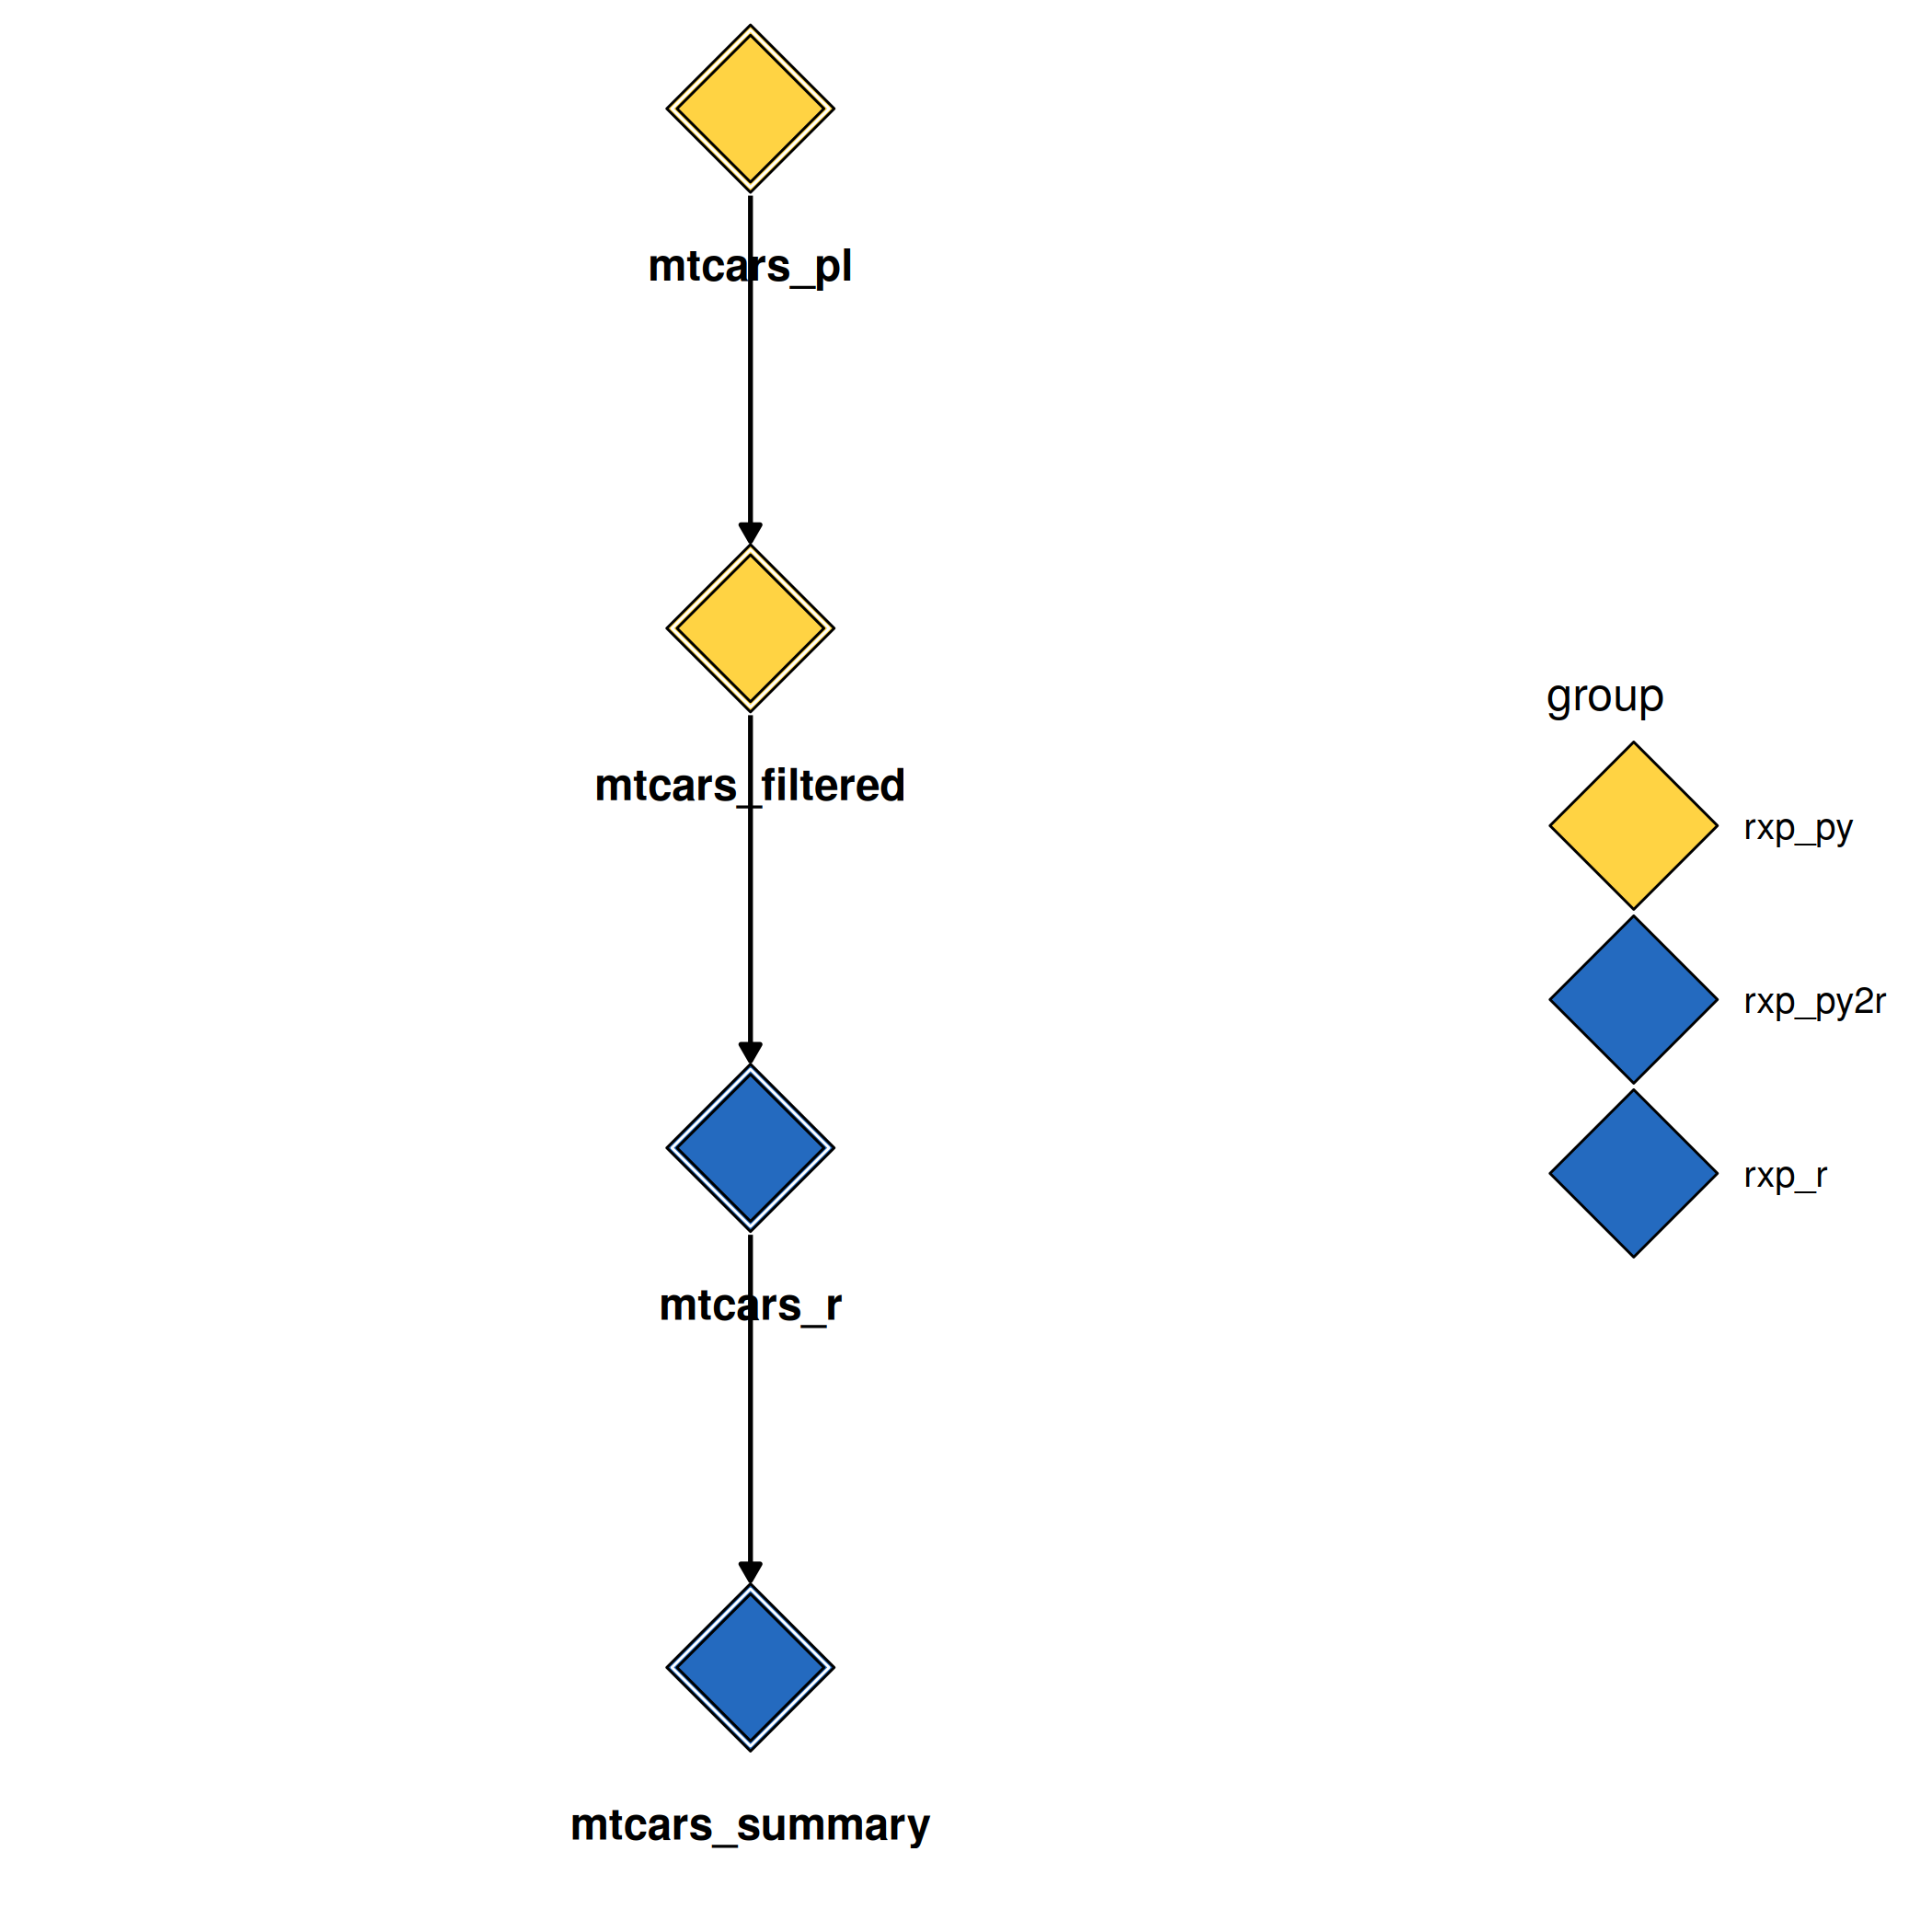
\includegraphics[keepaspectratio]{dag.png}}

}

\caption{Graphical representation of the pipeline}

\end{figure}%

Running the script above does not execute the pipeline; it generates a
\texttt{pipeline.nix} file, which declaratively defines the workflow.

To build and execute the pipeline:

\begin{CodeInput}
R> rxp_make()
\end{CodeInput}

\begin{CodeInput}
Build process started...

+ mtcars_pl building
+ mtcars_filtered building
+ mtcars_r building
+ mtcars_summary building
✓ mtcars_filtered built
✓ mtcars_pl built
✓ mtcars_r built
✓ mtcars_summary built
✓ pipeline completed [4 completed, 0 errored]
Build successful! Run `rxp_inspect()` for a summary.
Use `rxp_read("derivation_name")` to read objects or
`rxp_load("derivation_name")` to load them into the global environment.
\end{CodeInput}

\pkg{Nix} executes each step in order, building dependencies as needed.
Outputs are cached, so subsequent runs only recompute steps with changed
inputs or code. The build process can also be executed in parallel, if
the the pipeline has independent branches. This provides the efficiency
of \pkg{targets} with multi-language support and bit-for-bit
reproducibility. Artifacts can be inspected interactively in
\proglang{R} using \texttt{rxp\_read("artifact\_name")} or
\texttt{rxp\_load("artifact\_name")}.

For Python users, a port called \pkg{ryxpress} allows building the same
pipelines and inspecting outputs from Python sessions.

\pkg{rixpress} includes several additional features not covered here for
the sake of brevity.

It is also possible to configure popular IDEs to work interactively and
seamlessly with both \pkg{rix} and \pkg{rixpress}, enabling a smooth,
reproducible workflow from within the development environment. Detailed
setup instructions are provided in the vignettes of both packages.

\section{Conclusion}\label{sec-conclusion}

Many tools exist to improve reproducibility, but \pkg{Nix} stands out
because it deploys complete software environments \emph{closed under the
``depends on'' relation}: it installs not only a package, but all its
dependencies and their dependencies. This makes \pkg{Nix} particularly
powerful for reproducible research.

However, solving such a complex problem makes \pkg{Nix} a complex tool.
With \pkg{rix}, we aim to make \pkg{Nix} more accessible to \proglang{R}
users by providing a familiar interface and workflow. By building
reproducible development shells with \pkg{Nix}, researchers can
accommodate a wide range of use cases: running scripts and pipelines,
developing interactive \pkg{shiny} applications, or serving
\pkg{plumber} APIs.

Furthermore, \pkg{rixpress} extends this reproducibility to entire
analysis pipelines. By leveraging Nix as a build automation engine,
\pkg{rixpress} allows polyglot workflows where each step runs in its own
hermetically sealed environment. This ensures deep reproducibility,
efficient caching, and seamless orchestration of multi-language
analyses, making it easier to manage complex projects with confidence
that results can be reproduced exactly.

\section*{Acknowledgments}\label{acknowledgments}
\addcontentsline{toc}{section}{Acknowledgments}

We thank the rOpenSci reviewers and contributors who provided valuable
feedback on the development of \pkg{rix} and \pkg{rixpress}. In
particular, we are grateful to David Watkins and Jacob Wujiciak-Jens for
their reviews of \texttt{\{rix\}}, and to William Landau and Anthony
Martinez for their reviews of \texttt{\{rixpress\}}. We also acknowledge
the contributions of Richard J. Acton, Jordi Rosell, Elio Campitelli,
László Kupcsik, and Michael Heming for \texttt{\{rix\}}. Their expertise
and feedback greatly improved the quality and usability of these
packages.

\section*{References}\label{references}
\addcontentsline{toc}{section}{References}

\renewcommand{\bibsection}{}
\bibliography{bibliography.bib}





\end{document}
